
\lettrine[lines=3]{T}{}he string interpreter is one of the significant components of plant generation. It is the final step in the process of procedural generation. The output of this stage is dependant on what the L-system is representing. In this case, it is responsible for creating the final plant models and information and then rendering it on the screen, using the OpenGL framework. 

The interpreter has three main stages of processing, which can be seen in figure \ref{l-system interpreter}. The first part is the turtle graphics interpreter, then the model generator, and finally, the renderer. The turtle graphics interpreter takes the string of modules provided by the rewriter, as a set of instructions. It starts from the root of the tree and generates a skeletal structure made up of joints. This is similar to the techniques used in skeletal rigging in animation \cite{gregory2014game}. The tree skeleton joints each represent a branch segment or part of the tree. These joints have some information about the properties of that segment. The joint data is then used to generate the model data in the second stage of processing. The model generator creates the points that make up the plant in 3D space, as well as calculating the texture and lighting information. The models can finally be passed to the renderer. The renderer is responsible for taking all the model information such as, vertex, texture, and lighting data and renders the final plant on the screen. The renderer will also handle any physical simulation of the tree skeleton.

\begin{figure}[htbp]
	{\centering
		\vspace{7px}
		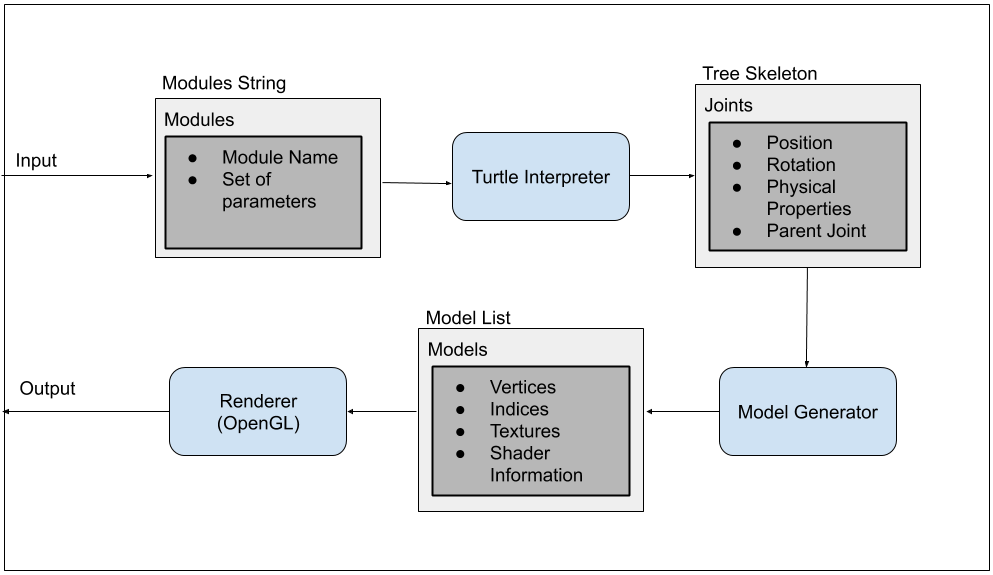
\includegraphics[scale=0.4]{Diagrams/L-systemInterpreter.png}
		\caption{Diagram of the stages of L-system interpretation and rendering} \label{l-system interpreter}
	}
\end{figure}
\FloatBarrier

\noindent
This chapter will cover each stage of the string interpreter implementation in detail. This chapter will also introduce how the interpreter can simulate and animation the plants' movements under forces such as gravity and wind in real-time. 

\section{Turtle Graphics Interpreter}

The primary purpose of the turtle graphics interpreter is to take the string of modules from the L-system rewriter and interpret each module as a turtle graphics instruction. Each instruction carries out a particular job in creating the overall structure of the plant. This stage is purely to follow the turtle graphics instructions and generate the skeletal data of the plant for the next stage.

This section is an implementation of what was covered in section \ref{Interpreting DOL-system}. Where a turtle graphics interpreter was defined for a simple DOL-system, however, there are several differences. The main difference is that the L-system string being interpreted is a parametric L-system and, therefore, consists of modules and parameters. Despite these differences, the overall concept remains the same. Each module name within the L-systems resultant string represents a particular meaning to the turtle graphics interpreter. The meaning of the module names are predefined in the string interpreter system and are dependant on what the L-system is trying to represent. The L-system defined for this thesis allows each module to provide optional parameters. These parameters may also carry particular meanings for the interpreter. For instance, the forward instruction or module name \say{F} can have three parameters. The value of the first parameter is the distance to move forward. The second and third parameter is the spring constant of the branch and the mass of the branch, respectively. These are useful in a physics simulation in order to animate the plant. 

Below is a table describing the L-system module names as well as the parameter meanings for the turtle graphics interpreter. In all of the instructions, there is also the case where no parameter is provided. This is still valid; however, if no parameter value is provided, a default value will be used.

\begin{table}[h!]
\centering
\begin{tabular}{ | c | l | l | l |}
\hline
	Instruction Name  & Meaning					& Parameter 1 	& Parameter 2 					\\  
\hline
\hline
	F 				&	Forward (Render)		& Length		& Spring Constant				\\
\hline
	f 				&	Forward (Don't render)	& Length 		& Spring Constant				\\
\hline
	+ 				&	Yaw	Right				& Angle 		&	N/A							\\
\hline
	- 				&	Yaw Left				& Angle			&	N/A							\\
\hline
	/ 				&	Pitch Up				& Angle			&	N/A							\\
\hline
	$\backslash$ 	&	Pitch Down				& Angle			&	N/A							\\
\hline
	$\land$ 		&	Roll Right				& Angle			&	N/A							\\
\hline
	\& 				&	Roll Left				& Angle 		&	N/A							\\
\hline
	! 				&	Change Width			& Branch Width	&	Resolution of Branch		\\
\hline
	[ 				&	Save State				& N/A			&	N/A							\\
\hline
	] 				&	Load State				& N/A 			&	N/A							\\
\hline
\end{tabular}
\caption{Table of turtle instruction symbols and their meaning to the interpreter}
\label{instruction table 1}
\end{table}
\FloatBarrier

\noindent
Each modules' instruction is carried out one by one to generate the plants' skeletal structure. The skeleton starts without any joints at the root location. All of the rotation instructions change the current angle of the turtle, and the change width instruction changes the value of its width. When one of the forward instructions is reached, a joint is created and added to the plants' skeleton. The joints hold information about the properties of each particular segment or object of the plant. The joints properties are the position, orientation, scale, parent joint, as well as its physical characteristics. It is important to note that all of the rotation and scale transforms must happen before the forward movement. A joint holds the properties seen in the diagram below.

\begin{figure}[htbp]
	{\centering
		\vspace{7px}
		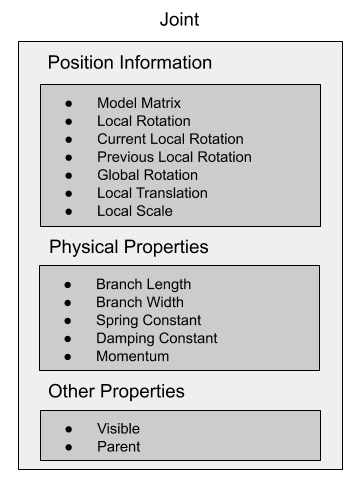
\includegraphics[scale=0.6]{Diagrams/JointDiagram.png}
		\caption{Diagram for the properties of a joint} \label{joint properties}
	}
\end{figure}
\FloatBarrier

\noindent
Figure \ref{joint properties} shows that there is a large amount of information stored for the position and orientation of each joint. This is because the rotation of the joint is stored in both a local and global space. Local space refers to the rotation of the joint relative to its parent rotation. This is useful as it allows the manipulation of subsequent child joints while leaving other joints local rotation unchanged. Global space, also known as world space, is the rotation of each joint relative to the world itself. This is useful for understanding the current rotation of the joint relative to the world. It is essential to store both the current and previous rotations as they are used to calculate the rate of change for physics calculations.

The physical properties for each joint are the parts that will affect model generation as well as physics simulations. These properties include the length, width, spring constant, damping constant as well as the current momentum of the branch. 

Take the following string of modules \say{F(1)[/(90)F(1)$\backslash$ (90)F(1)]-(90)F(1)+(90)F(1)}, the alphabet is made up of seven unique modules F, /, $\backslash$, [, ], + and -. As discussed in previous chapters the \say{F} symbol represents a move forward, and \say{+}, \say{-}, \say{/}, \say{$\backslash$} symbolize different rotations, and the \say{[} and \say{]} represent save and load state respectively. The symbols in the string above each have a single parameter except the load and save state. It is the turtle graphics interpreters' job to understand what these parameters are and how to interpret them. In this case, all of the \say{F} modules have the parameter value of 1, and all of the rotation modules have the parameter of 90. These are interpreted as the length to move forward and the change in angle from the previous joint. This interpretation can be displayed with the joint structure shown in figure \ref{skeleton diagram} below.

\begin{figure}[htbp]
	{\centering
		\vspace{7px}
		\setlength{\fboxrule}{1pt}
		\fbox{
			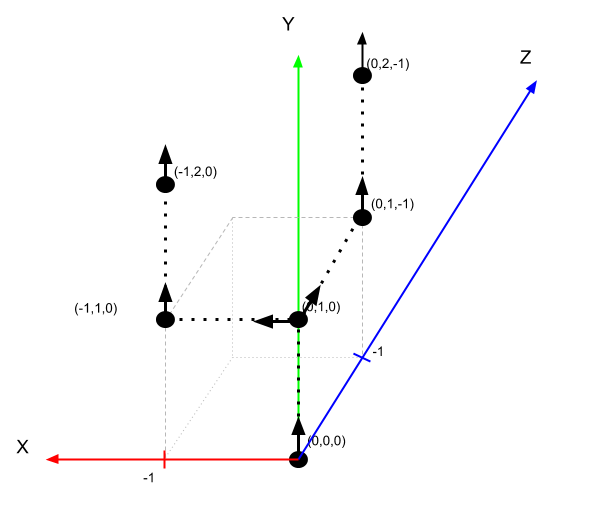
\includegraphics[scale=0.4]{Diagrams/SkeletonJoints.png}
		}
		\caption{Diagram of a simple plant skeleton with joint position and orientation.} \label{skeleton diagram}
	}
\end{figure}
\FloatBarrier

\noindent
Once the plant skeleton containing all of the joints has been created, the model generator can use this information to create the geometry of the plants' branches and leaves. Something to note is that there are two separate joints at the position (0, 1, 0), this is due to the fact that there are two branches going in different directions with independent features such as, width or length. 

\section{Model Generator}

Modeling the branches of a plant is one of the most critical parts of the look and feel of the plant being generated. The plant skeleton and joints describe details about the plants' structure. The job of the model generator is to take the skeleton information and intelligently generate the 3D models' that make up the plants' branches, leaves, or flowers. The models of these objects are made up of vertices, normals, texture coordinates, and other low-level information that can then be provided to the OpenGL renderer and finally displayed on the screen using the GPU.

There are many different ways of procedurally modeling the branching branches of a plant. The simplest would be to take several cylinders, rotate and stack them according to each joints position in 3D space. The upside to this approach that it is very efficient, as every branch within the plant shares the same object model, which is a cylinder. This method can approximate the branching structure of the plant. However, there is a problem, which was pointed out by Baele and Warz\'{e}e ``The branches junction causes a continuity problem: to simply stack up cylinders generates a gap'' \cite{baele2005real}. The continuity problem can be seen in the figure below.

\begin{figure}[htbp]
	{\centering
		\vspace{7px}
		\setlength{\fboxrule}{1pt}
		\fbox{
			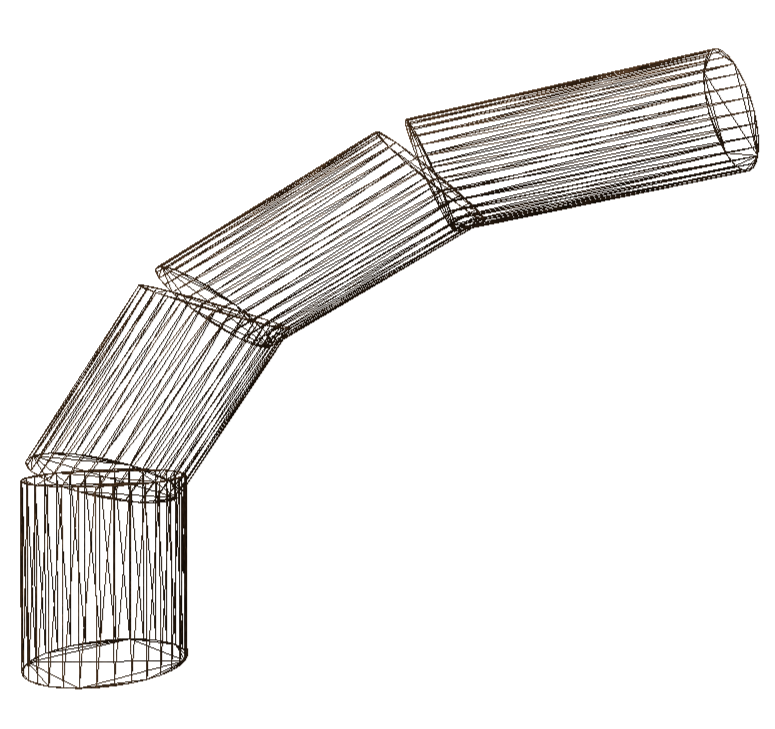
\includegraphics[scale=0.2]{Diagrams/stackedBranchesMesh.png}
		}
		\caption{Example of the continuity problem faced with stacked branching with a 25$^{\circ}$ bend per joint.}
	}
\end{figure}

\FloatBarrier

\noindent
The simple method of stacking cylinders gives an approximation of the tree structure. It is usually a good enough representation when the branch angles are not more than 25$^{\circ}$, and the size of the branches do not change. However, for a much more convincing tree structure, there will need to be a better solution. 

An improvement would be to link all of the branch segments together to make the entire branching structure seamless. The top vertices from the parent branch must be linked with the bottom of its child branch. The vertices that make up the top and bottom of a branch are circles of vertices, which are linked together using indexing. These circles will have to rotate depending on the bending direction of the branch. This means that the final model will not be made up of a large number of the same model but rather a single large model. 

There are several points to keep in mind for linked branching. The first is that this process is much less efficient than rendering the same cylindrical object many times. The reason for this is that every vertex within the tree needs to be calculated, generated, and finally linked. The second point is what happens when there are multiple branches off a single joint. This will be covered in more detail later. The final point has to do with the resolution of the branch. The resolution is the number of points making up the circumference of the branch. The resolution can be increased or decreased as needed. A higher resolution plant might look better but will also be more resource-intensive to render. Conversely, a lower resolution plant might look a bit more jagged, but be far less resource-intensive to render. An example of the linked branching can be seen below.

\begin{figure}[htbp]
	{\centering
		\vspace{7px}
		\setlength{\fboxrule}{1pt}
		\fbox{
			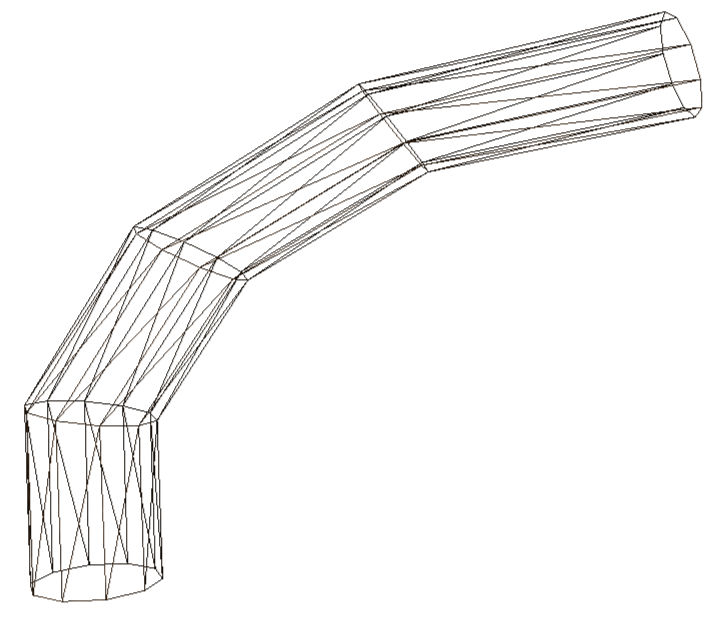
\includegraphics[scale=0.2]{Diagrams/linkedBranchesMesh.png}
		}
		\caption{Example of linked branching with a 25$^{\circ}$ bend per joint.}
	}
\end{figure}
\FloatBarrier

\noindent
This method of branch generation, at first glance, gives a very similar result to that of stacking cylinders. Although it does have a few advantages, firstly, it completely avoids the branch gap problem when there are larger angle changes, as well as branch size changes. As discussed previously, the second advantage is that the resolution is dynamic. This can be seen in figure \ref{stackedvslinked} below, where a similar-looking branch can be achieved using less than half the number of vertices, with joined branches instead of stacked branches.


\begin{figure}[htbp]
	{\centering
		\vspace{7px}
		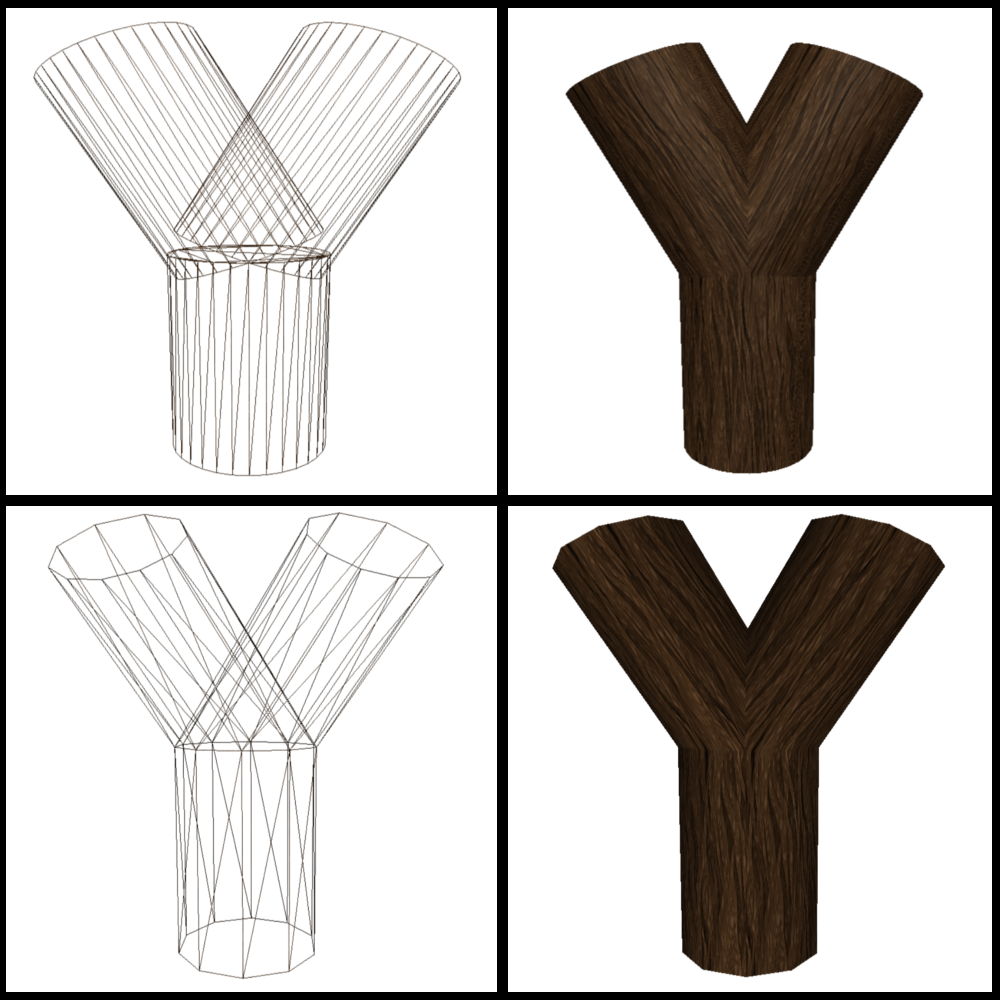
\includegraphics[scale=0.2]{Diagrams/StackedVsLinked.png}\label{stackedvslinked}
		\caption{Stacked Vs Linked.}
	}
\end{figure}
\FloatBarrier

This technique of linking branches can be further improved by creating curvature from one branch to the next and by adding a smoothed noise function to the vertices that make up the branches. The advantage of this is that the branches have additional complexity and texture, which makes them look more realistic than the simple linking approach. However, the drawback is that they are more complicated to generate and more resource-demanding to render \cite{baele2005real}.

\section{Renderer}

\noindent
The renderer is the final stage in the procedural generation pipeline. It takes all of the 3D models generated by the model generator, such as leaves, branches, flowers, and renders them on the screen.  For this thesis, \acrshort{opengl} is use used to render the models on the screen using the \acrshort{gpu} efficiently. 

The \acrshort{gpu} is a specially designed piece of hardware for processing computer graphics and image processing. It has hundreds or even thousands of individual compute cores that can be used in parallel. Due to the highly parallel nature of the \acrshort{gpu}, the \acrshort{opengl} framework helps to abstract the hardware and create an interface to interact with the \acrshort{gpu} in a more straightforward way. There are several other types of graphics \acrshort{api}, such as Vulkan, Metal, or DirectX. These \acrshort{api}s all provide a way of interacting with the hardware behind the scenes. However, they each have a different approach. Therefore, this section will not be going into great detail about the specifics of \acrshort{opengl} but rather the general concepts required for rendering the plant model on the screen. The main parts of the rendering stage have to do with how model data is stored into buffer objects, secondly how textures are stored and then mapped to a specific object and thirdly how lighting can be calculated for a procedurally generated object.

\subsection{Models and Buffer Objects}

The model generator produces all of the information necessary for the renderer to produce the result on the screen. In general, the model data will consist of vertex data, texture coordinates, and vertex normals. The vertex data is simply the position of a point within the model, three vertices make up a face, and the faces are ultimately rendered on the screen. The texture coordinates are the locations on a texture image that maps directly to the model vertices, in order to have a textured object in the scene. Finally, the vertex normals, known as normals, are the average normal vector. A normal vector is a vector that is perpendicular to the surface at a given point and can be used for Phong shading or other types of lighting techniques.  

One of the most important parts of the rendering process is buffering the model data onto the \acrshort{gpu}. The \acrlong{vbo} (\acrshort{vbo}) is a data structure within the \acrshort{opengl} library which can be used to store this data on the \acrshort{gpu}. Generally, the data is stored as a single buffer or array with the first three values being a vertex position, the second two being a texture coordinate, and the last three being a vertex normal.

\begin{figure}[htbp]
	{\centering
		\vspace{7px}
		\setlength{\fboxrule}{1pt}
		\fbox{
			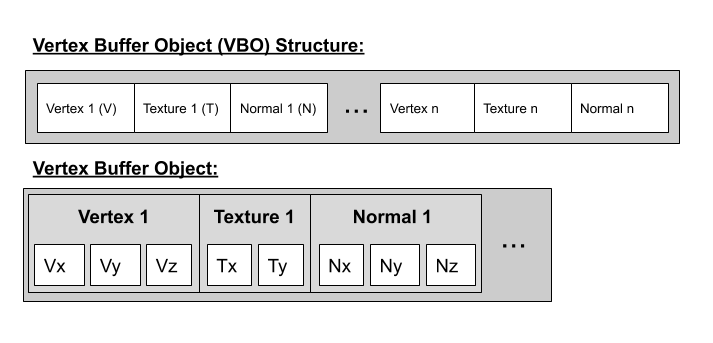
\includegraphics[scale=0.5]{Diagrams/VertexObjects.png}
		}
		\caption{Diagram showing the structure of a vertex buffer object.}
	}
\end{figure}
\FloatBarrier

\noindent
Buffer objects can be created not only for the plant branching structure but potentially for different parts of the plant, for instance, leaves or flowers. The leaves and flowers on a single tree tend to be very similar, so there is no need to have thousands of copies of a leafs' model or texture. This would be highly wasteful and unnecessary. Instead, there could be one copy of the vertex data, and texture data and instanced rendering can be used to render many copies of this single object in different places on the plant. 

\section{Shaders}

A shader is type of computer program which is used for shading an object within a 3D scene. The shader program typically runs on the GPU and calculates the levels of colour and lighting for a specific part of an object within the scene. More modern types of shading can be used to provide effects like tesselation. 

\section{Summary}

This chapter outlines the implementation of the string interpreter for representing plant-life. This consists of a three-stage process, firstly the resulting string from the rewriter is interpreted using turtle graphics to generate the skeletal structure of the plant, which is made up of joints. The model generator then uses the skeletal structure as a frame for creating the plants' branch model data. The plants' model data is finally passed to the renderer, which draws the resulting image on the screen. 

Each branch joint contains a large amount of data that is used when rendering the plant and physics calculations. The way that the model generator creates and links branches can easily be changed, modified, or improved to generate different types of branches. In this thesis, two methods are covered, the stacked cylinders technique and linked branches. 

The renderer is very platform dependent but usually takes place on the GPU, where buffer objects are used to store the plants model data in GPU memory and eventually displayed through the use of shaders.







